\documentclass[]{beamer}
\mode<presentation>
{
\usetheme{-bjeldbak/beamerthemebjeldbak}
  \usecolortheme{default} % or try albatross, beaver, crane, ...
  \usefonttheme{default}  % or try serif, structurebold, ...
\usepackage[english]{babel}
\usepackage[utf8x]{inputenc}
 \usepackage{subfiles}
\setbeamertemplate{caption}{\insertcaption}
  \setbeamertemplate{navigation symbols}{}
  \setbeamertemplate{caption}[numbered]
\setbeamertemplate{navigation symbols}[horizontal]
} 

\begin{document}
 \graphicspath{{images/}}

\title{Innappropriate parameterzation of fossilized birth-death models causes incorrect estimates of topology and node ages}
\author{April M. Wright \\ Tracy A. Heath}
\date{Today}
\maketitle

\begin{frame}
\frametitle{Outline}
\begin{itemize}
\item Overview: The Fossilized-Birth Death Process
\item Our Research Question
\item Methods
\item Results
\end{itemize}
\end{frame}


\begin{frame}
\frametitle{Fossilized Birth-Death Process}
\end{frame}

\begin{frame}
\frametitle{Fossilized Birth-Death Process}
\begin{itemize}
\item A probabilistic model for estimating divergence times
\end{itemize}
\end{frame}

\begin{frame}
\frametitle{Fossilized Birth-Death Process}
\begin{center}
\begin{tabular}{ l  | r }
Parameter & Meaning \\
\hline 
\lambda & Speciation Rate 
\end{tabular}
\end{center}
\end{frame}



\begin{frame}
\frametitle{Fossilized Birth-Death Process}
\begin{center}
\begin{tabular}{ l  | r }
Parameter & Meaning \\
\hline 
\lambda & Speciation Rate \\
\mu & Extinction Rate \\ 
\end{tabular}
\end{center}
\end{frame}

\begin{frame}
\frametitle{Fossilized Birth-Death Process}
\begin{center}
\begin{tabular}{ l  | r }
Parameter & Meaning \\
\hline 
\lambda & Speciation Rate \\
\mu & Extinction Rate \\ 
\psi & Paleo Sampling\\
\end{tabular}
\end{center}

\end{frame}

\begin{frame}
\frametitle{Fossilized Birth-Death Process}
\begin{center}
\begin{tabular}{ l  | r }
Parameter & Meaning \\
\hline 
\lambda & Speciation Rate \\
\mu & Extinction Rate \\ 
\psi & Paleo Sampling\\
\rho & Extant Sampling \\
\end{tabular}
\end{center}
\end{frame}

\begin{frame}
\frametitle{Fossilized Birth-Death Process}
\begin{itemize}
\item A probabilistic model for estimating divergence times
\item Treat fossil and molecular data as part of the same process
\end{itemize}
\end{frame}

\begin{frame}
\frametitle{Fossilized Birth-Death Process}
\begin{itemize}
\item A probabilistic model for estimating divergence times
\item Treat fossil and molecular data as part of the same process 
\begin{itemize}
	\item Avoid calibration densities 
	\item Use multiple fossils per node
\end{itemize}	
\end{itemize}
\end{frame}

\begin{frame}
\frametitle{Fossilized Birth-Death Process}
\begin{itemize}
\item A probabilistic model for estimating divergence times
\item Treat fossil and molecular data as part of the same process 
\begin{itemize}
	\item Avoid calibration densities 
	\item Use multiple fossils per node
\end{itemize}
\item Allow ancestors to be sampled 	
\end{itemize}
\end{frame}

\begin{frame}
\frametitle{Fossilized Birth-Death Process}
\begin{itemize}
\item A probabilistic model for estimating divergence times
\item Treat fossil and molecular data as part of the same process 
\begin{itemize}
	\item Avoid calibration densities 
	\item Use multiple fossils per node
\end{itemize}
\item \textbf{Allow ancestors to be sampled}	
\end{itemize}
\end{frame}

\begin{frame}
\frametitle{Divergence Dating and Reasonable Ages}
\end{frame}

\begin{frame}
\frametitle{Divergence Dating and Reasonable Ages}
\begin{itemize}
\item Empirical studies have noted that dated trees made using combined molecular+morphological data tend to produce older ages than studies with molecular data and node calibrations
\end{itemize}
\end{frame}

\begin{frame}
\frametitle{Divergence Dating and Reasonable Ages}
\begin{itemize}
\item Empirical studies have noted that dated trees made using combined molecular+morphological data tend to produce older ages than studies with molecular data and node calibrations
\end{itemize}
\end{frame}

\begin{frame}
\frametitle{Our Research Question}
Is this an inherent property of 'total-evidence' approaches, or is this related to model misspecification?
\end{frame}

\begin{frame}
\frametitle{Our Research Question}
Sampled ancestor models
\begin{figure}
Low turnover, high sampling  \\
Few sampled ancestors \\
\lambda   \mu   \psi   \rho \\
\includegraphics[scale=0.4]{images/HighTurnHighSamplog.png}
\end{figure}
\end{frame}

\begin{frame}
\frametitle{Our Research Question}
Sampled ancestor models
\end{frame}

\begin{frame}
\frametitle{Our Research Question}
Sampled ancestor models
\end{frame}

\begin{frame}
\frametitle{Methods}
\end{frame}

\begin{frame}
\frametitle{Methods}
\begin{itemize}
\item Simulations
\end{itemize}
\end{frame}

\begin{frame}
\frametitle{Methods}
\begin{itemize}
\item Simulations
\begin{itemize}
\item 25 extant tips with nucleotide sequence data
\item Variable number of fossil tips, with missing data
\end{itemize}
\end{itemize}
\end{frame}

\begin{frame}
\frametitle{Methods}
\begin{itemize}
\item Simulations
\begin{itemize}
\item 25 extant tips with nucleotide sequence data
\item Variable number of fossil tips, with missing data
\item Simulate different values for \lambda, \mu ,  \psi
\end{itemize}
\end{itemize}
\end{frame}

\begin{frame}
\frametitle{Methods}
\begin{itemize}
\item Empirical Data
\begin{itemize}
\item Bear data set of Heath et al. 2014.
\end{itemize}
\end{itemize}
\end{frame}

\begin{frame}
\frametitle{Methods}
\begin{itemize}
\item Estimation
\begin{itemize}
\item Estimate a tree for each dataset using both sampled ancestor and non-sampled ancestor models in BEAST2
\end{itemize}
\end{itemize}
\end{frame}

\begin{frame}
\begin{center}
\begin{figure}
Low turnover, low sampling  \\
Few sampled ancestors \\
\lambda   \mu   \psi   \rho \\
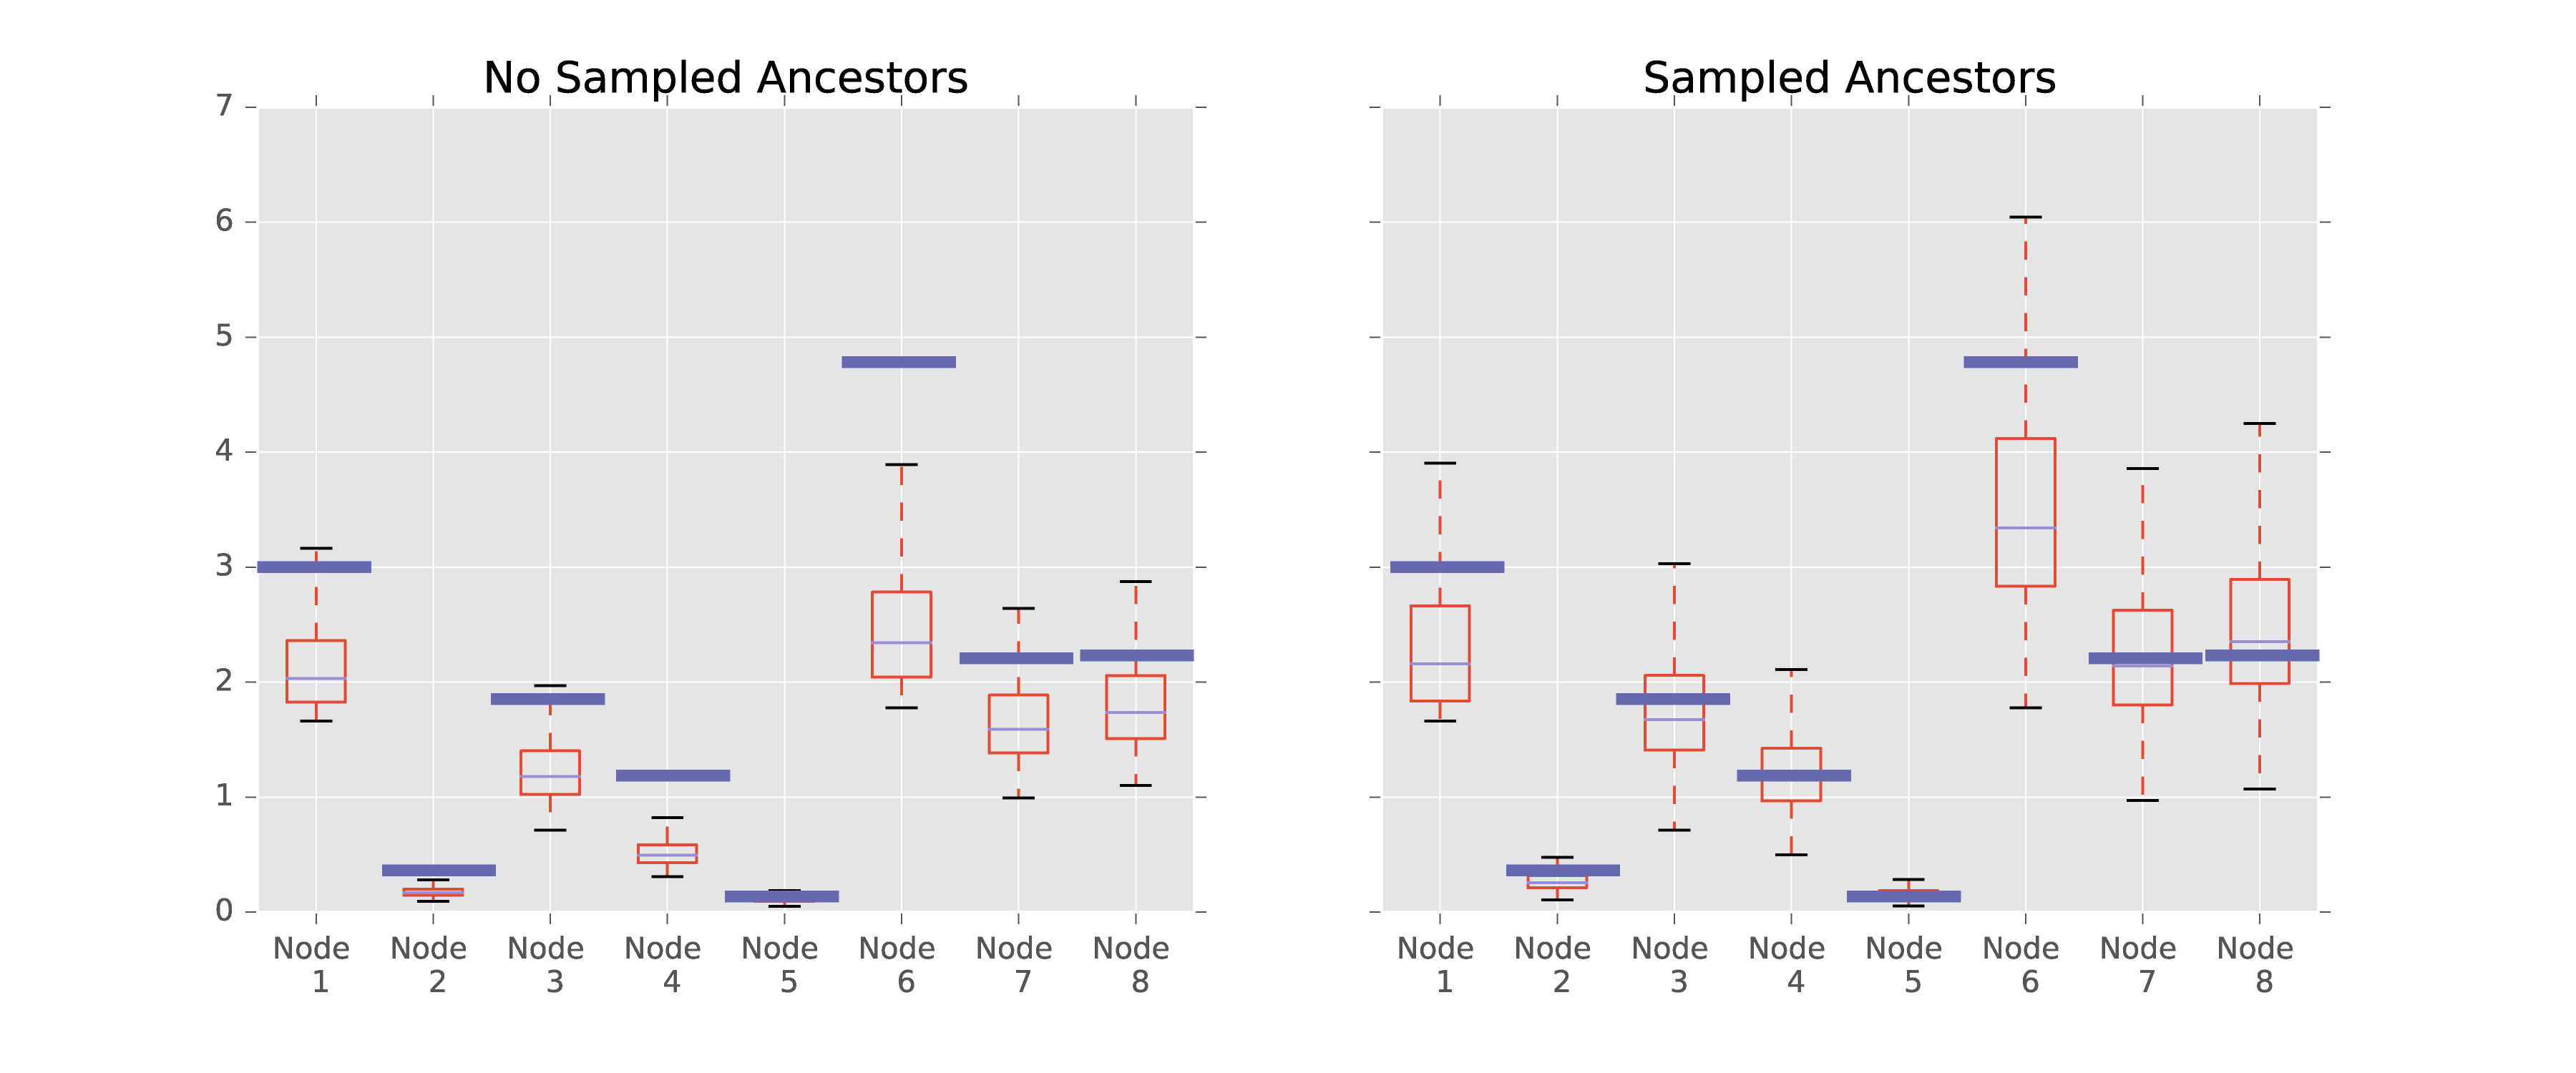
\includegraphics[scale=0.4]{images/LowTurnLowSampnodes.png}
\end{figure}
\end{center}
\end{frame}

\begin{frame}
\begin{center}
\begin{figure}
Low turnover, low sampling  \\
Few sampled ancestors \\
\lambda   \mu   \psi   \rho \\
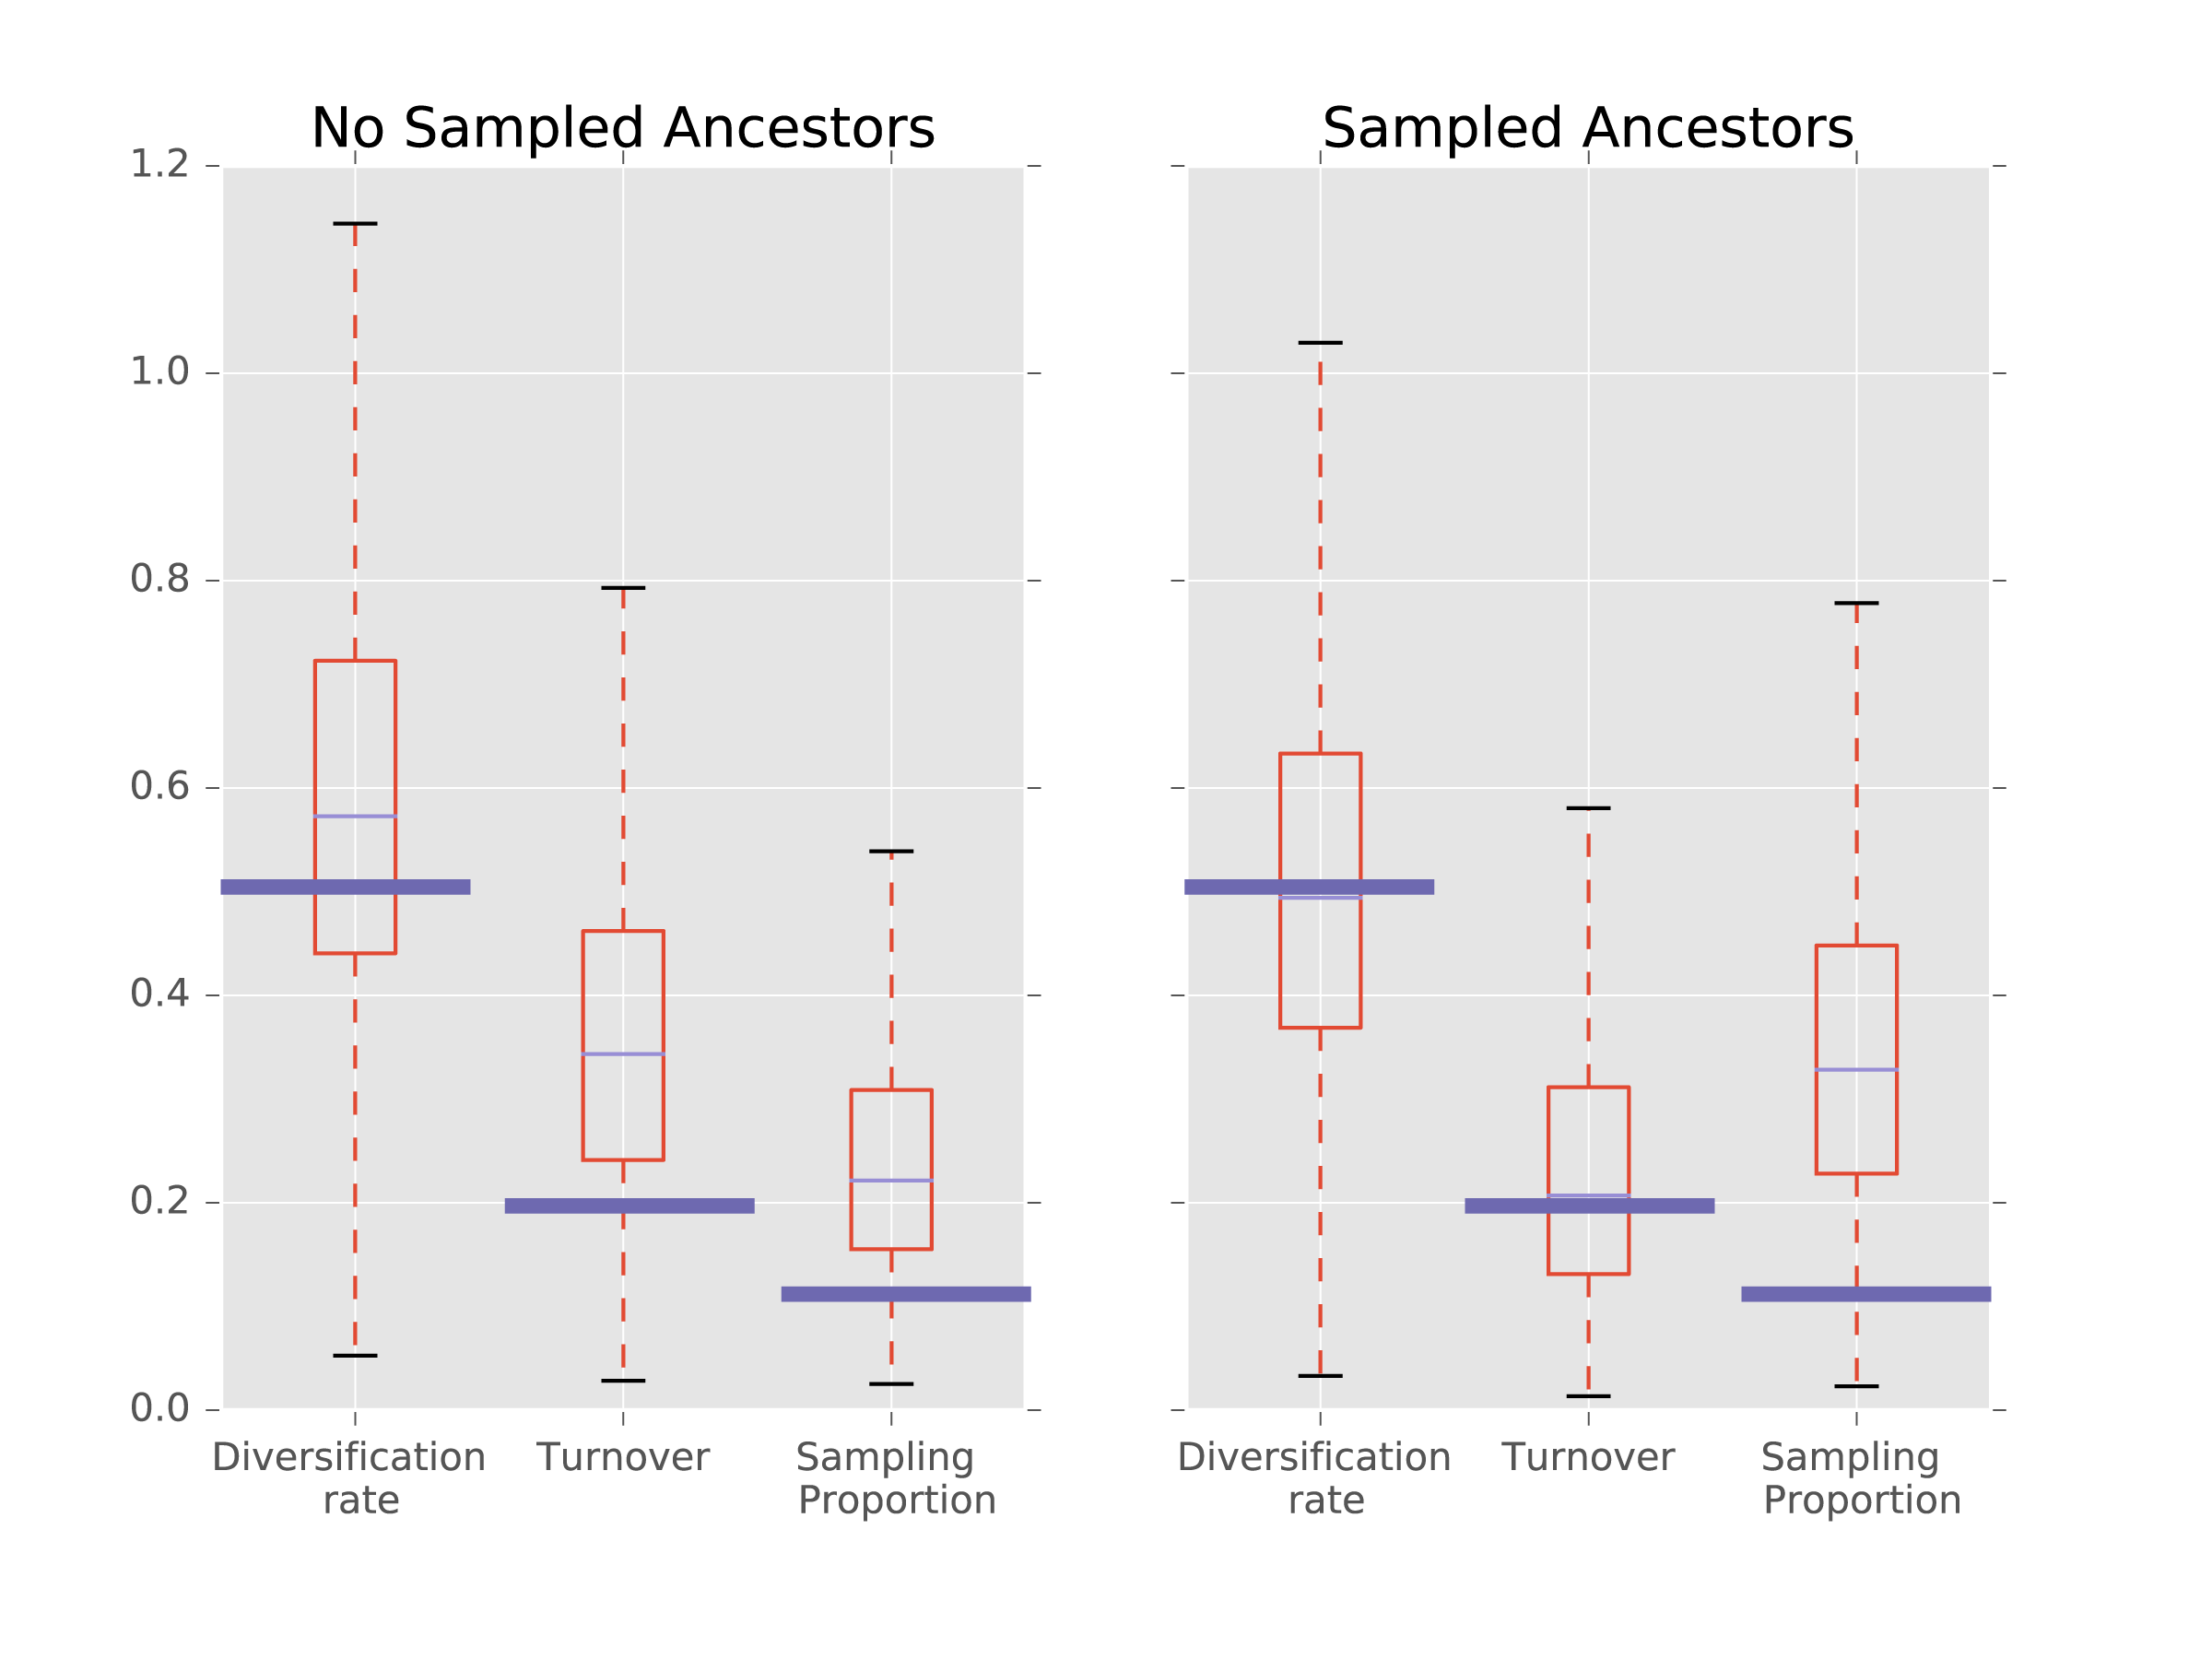
\includegraphics[scale=0.4]{images/LowTurnLowSamplog.png}
\end{figure}
\end{center}
\end{frame}


\begin{frame}
\frametitle{Results}
\begin{center}
\begin{figure}
Low turnover, high sampling  \\
Few sampled ancestors \\
\lambda   \mu   \psi   \rho \\
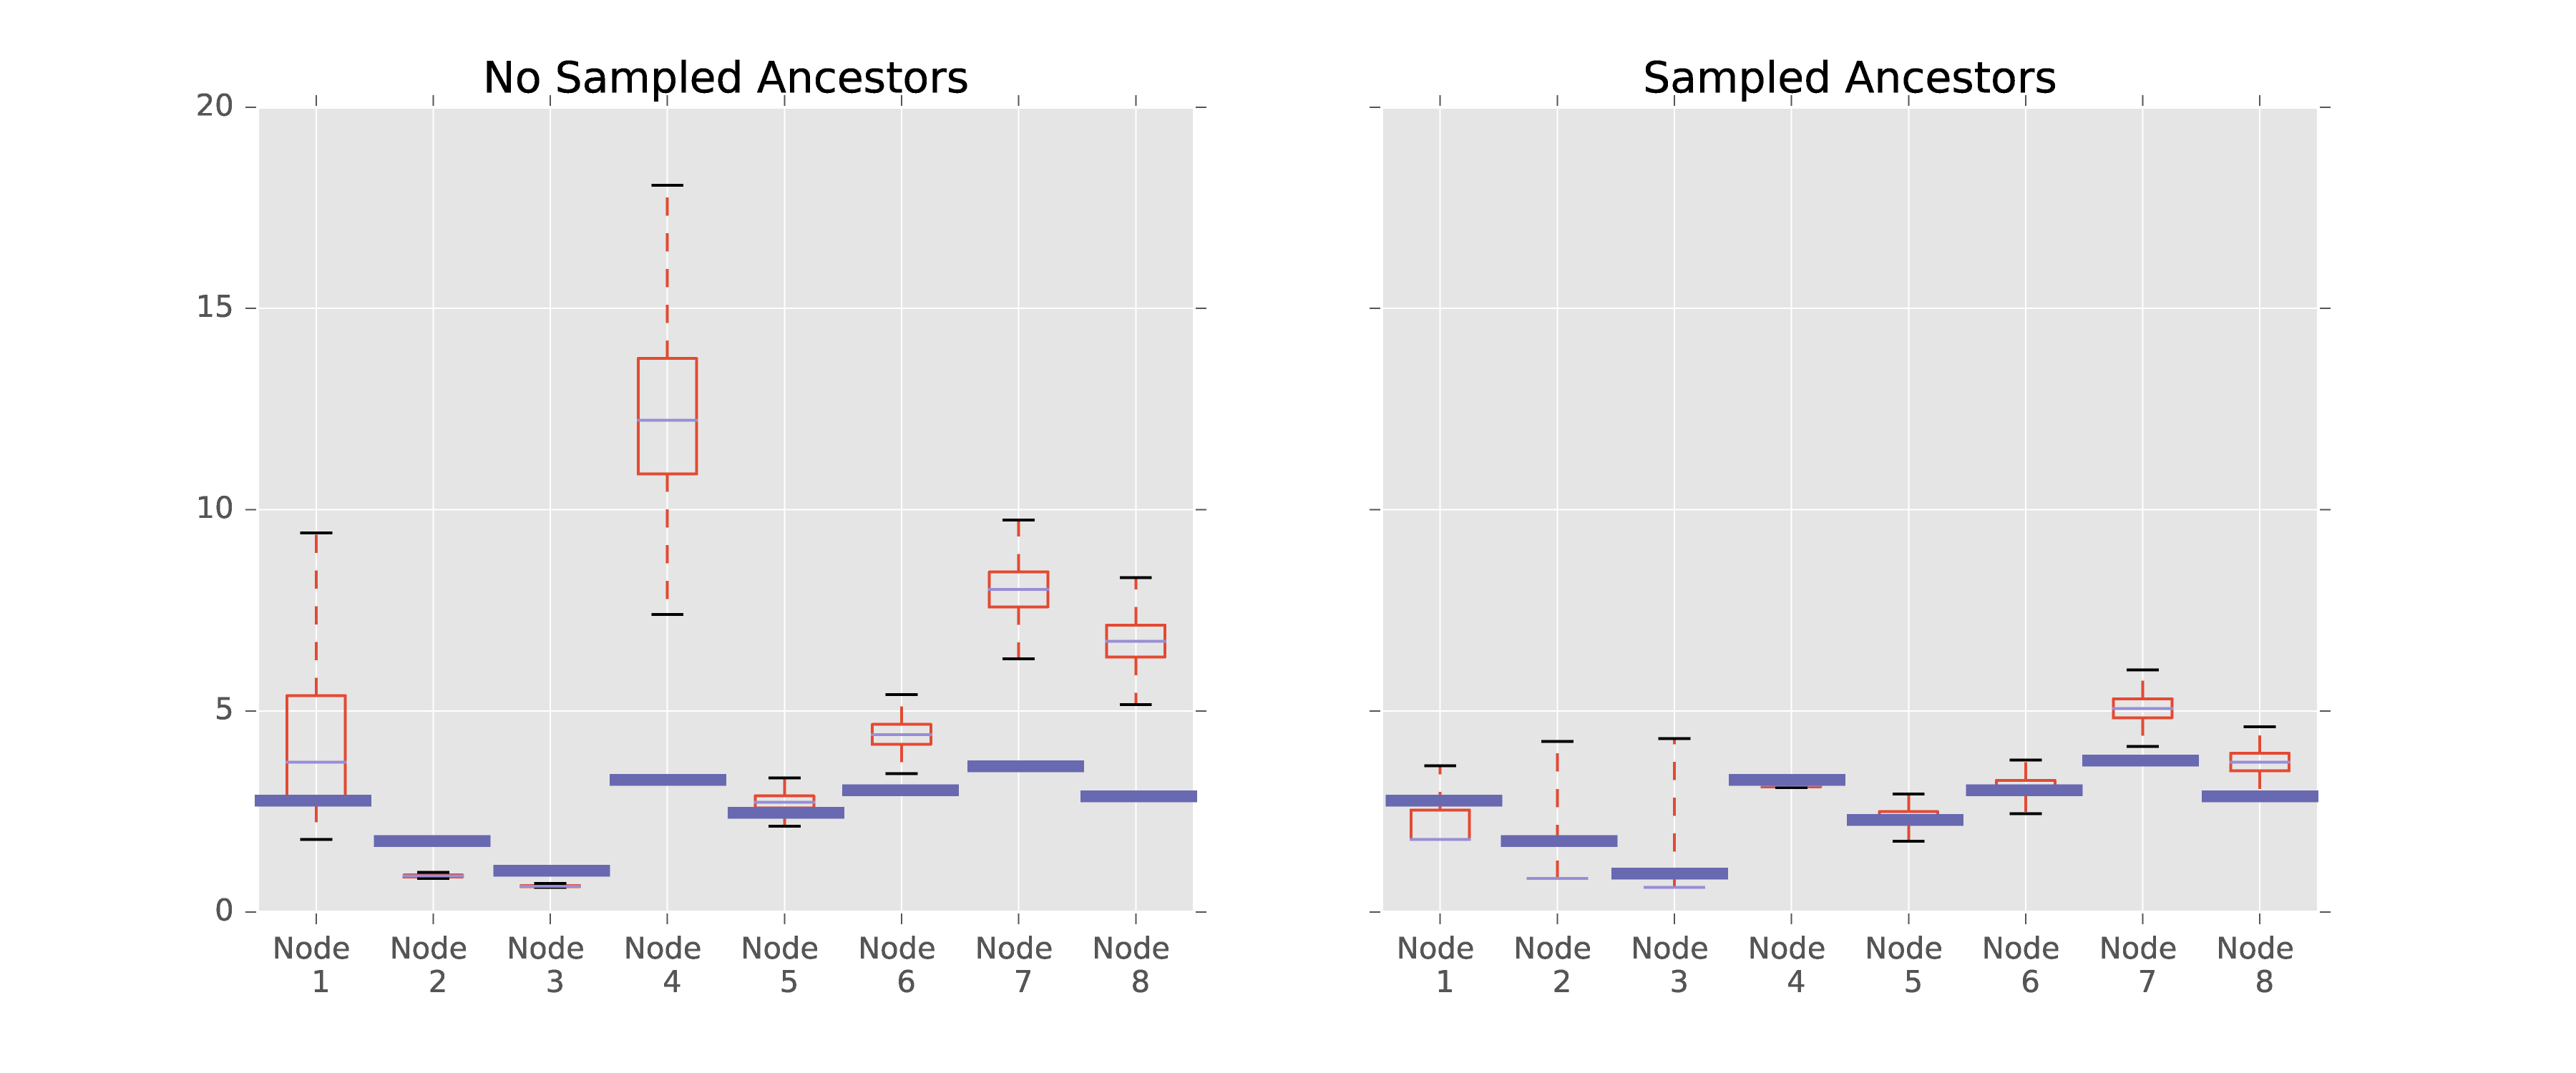
\includegraphics[scale=0.4]{images/LowTurnHighSampnodes.png}
\end{figure}
\end{center}
\end{frame}

\begin{frame}
\frametitle{Results}
\begin{center}
\begin{figure}
Low turnover, high sampling  \\
Few sampled ancestors \\
\lambda   \mu   \psi   \rho \\
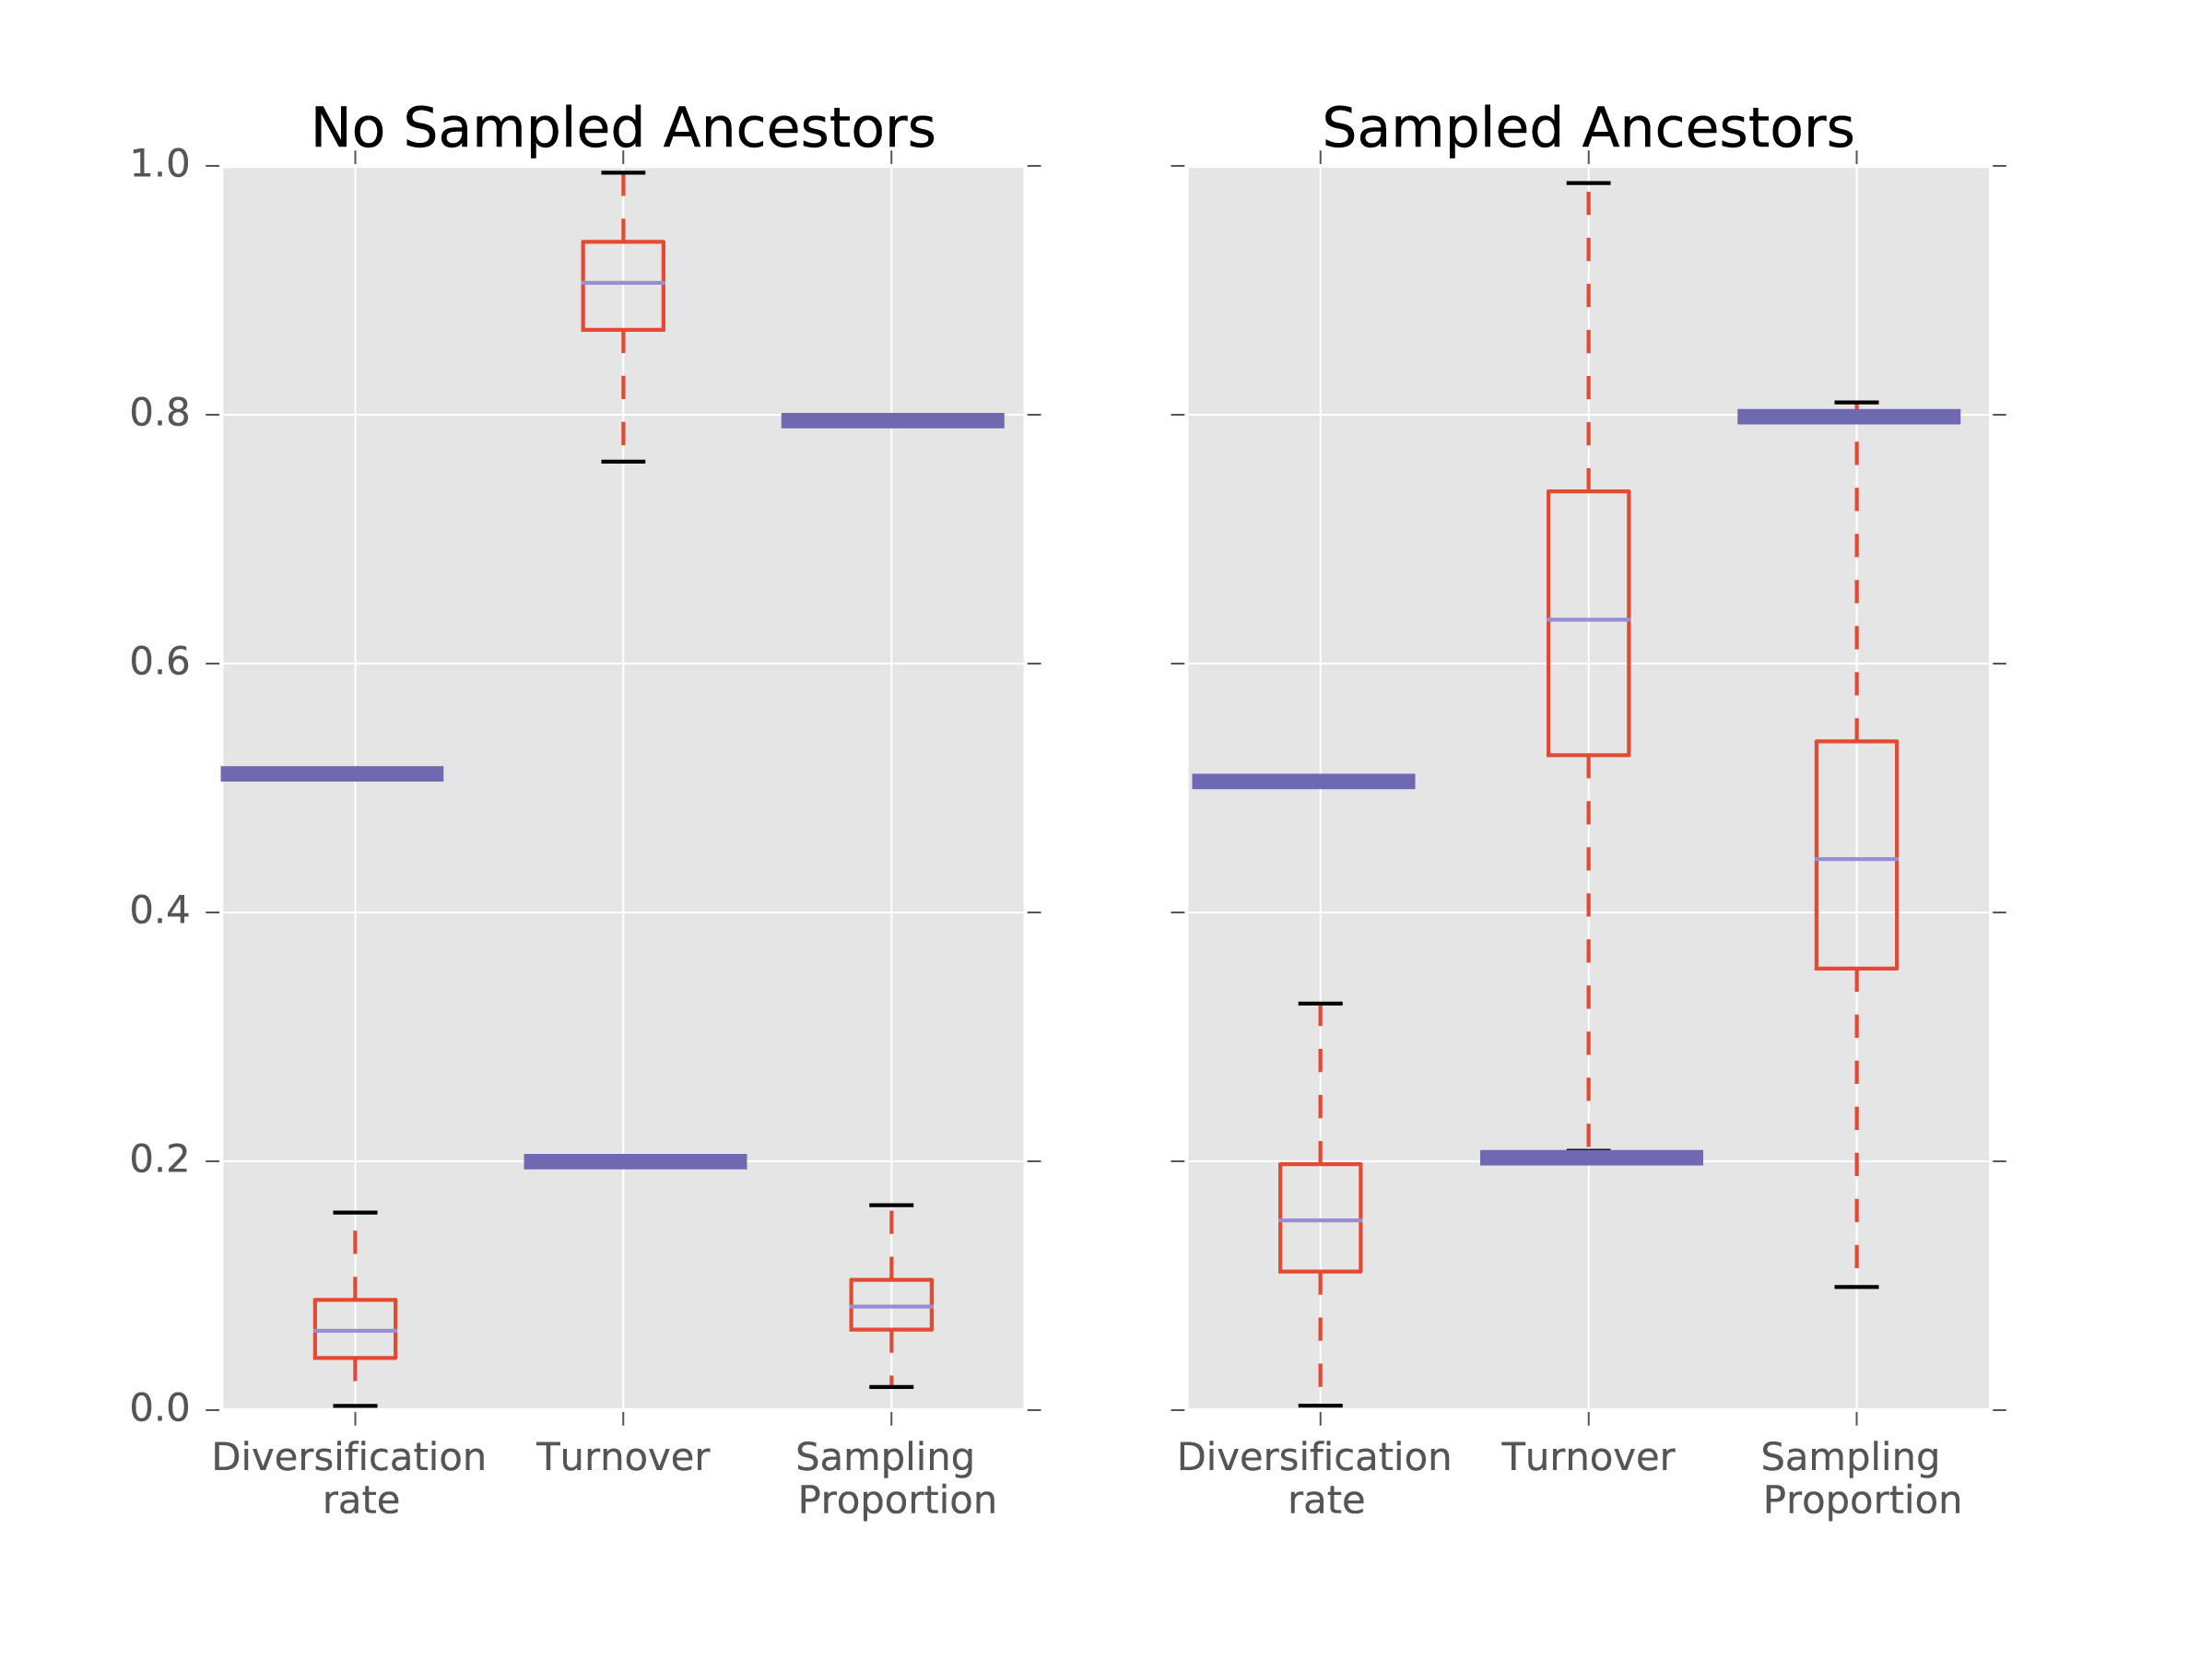
\includegraphics[scale=0.4]{images/LowTurnHighSamplog.png}
\end{figure}
\end{center}
\end{frame}

\begin{frame}
\begin{center}
\begin{figure}
High turnover, low sampling  \\
Few sampled ancestors \\
\lambda   \mu   \psi   \rho \\
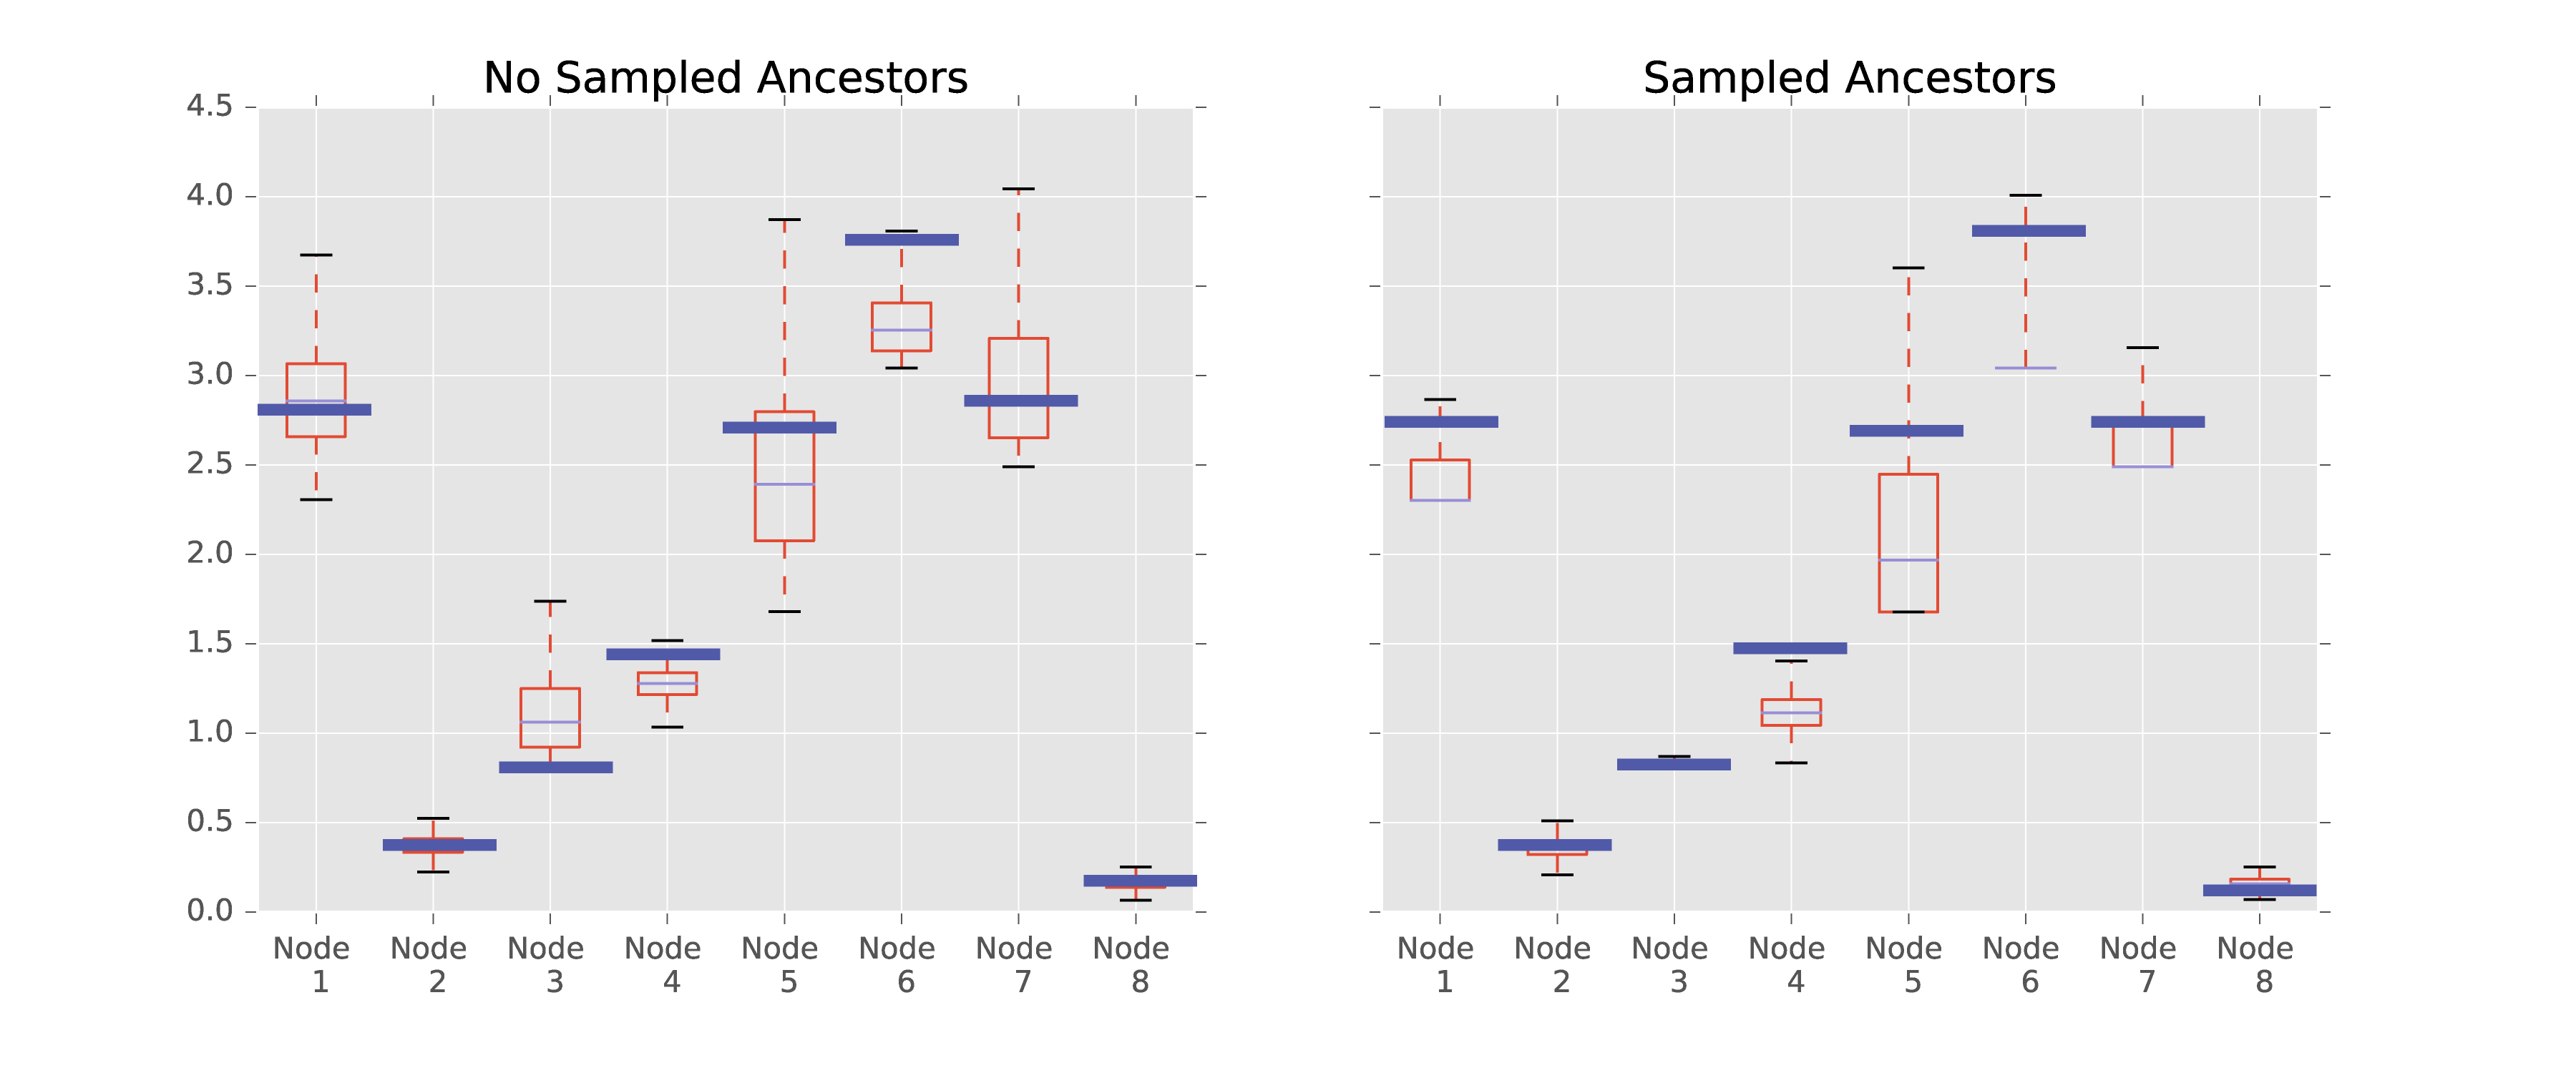
\includegraphics[scale=0.4]{images/HighTurnLowSampnodes.png}
\end{figure}
\end{center}
\end{frame}

\begin{frame}
\frametitle{Results}
\begin{center}
\begin{figure}
Low turnover, high sampling  \\
Few sampled ancestors \\
\lambda   \mu   \psi   \rho \\
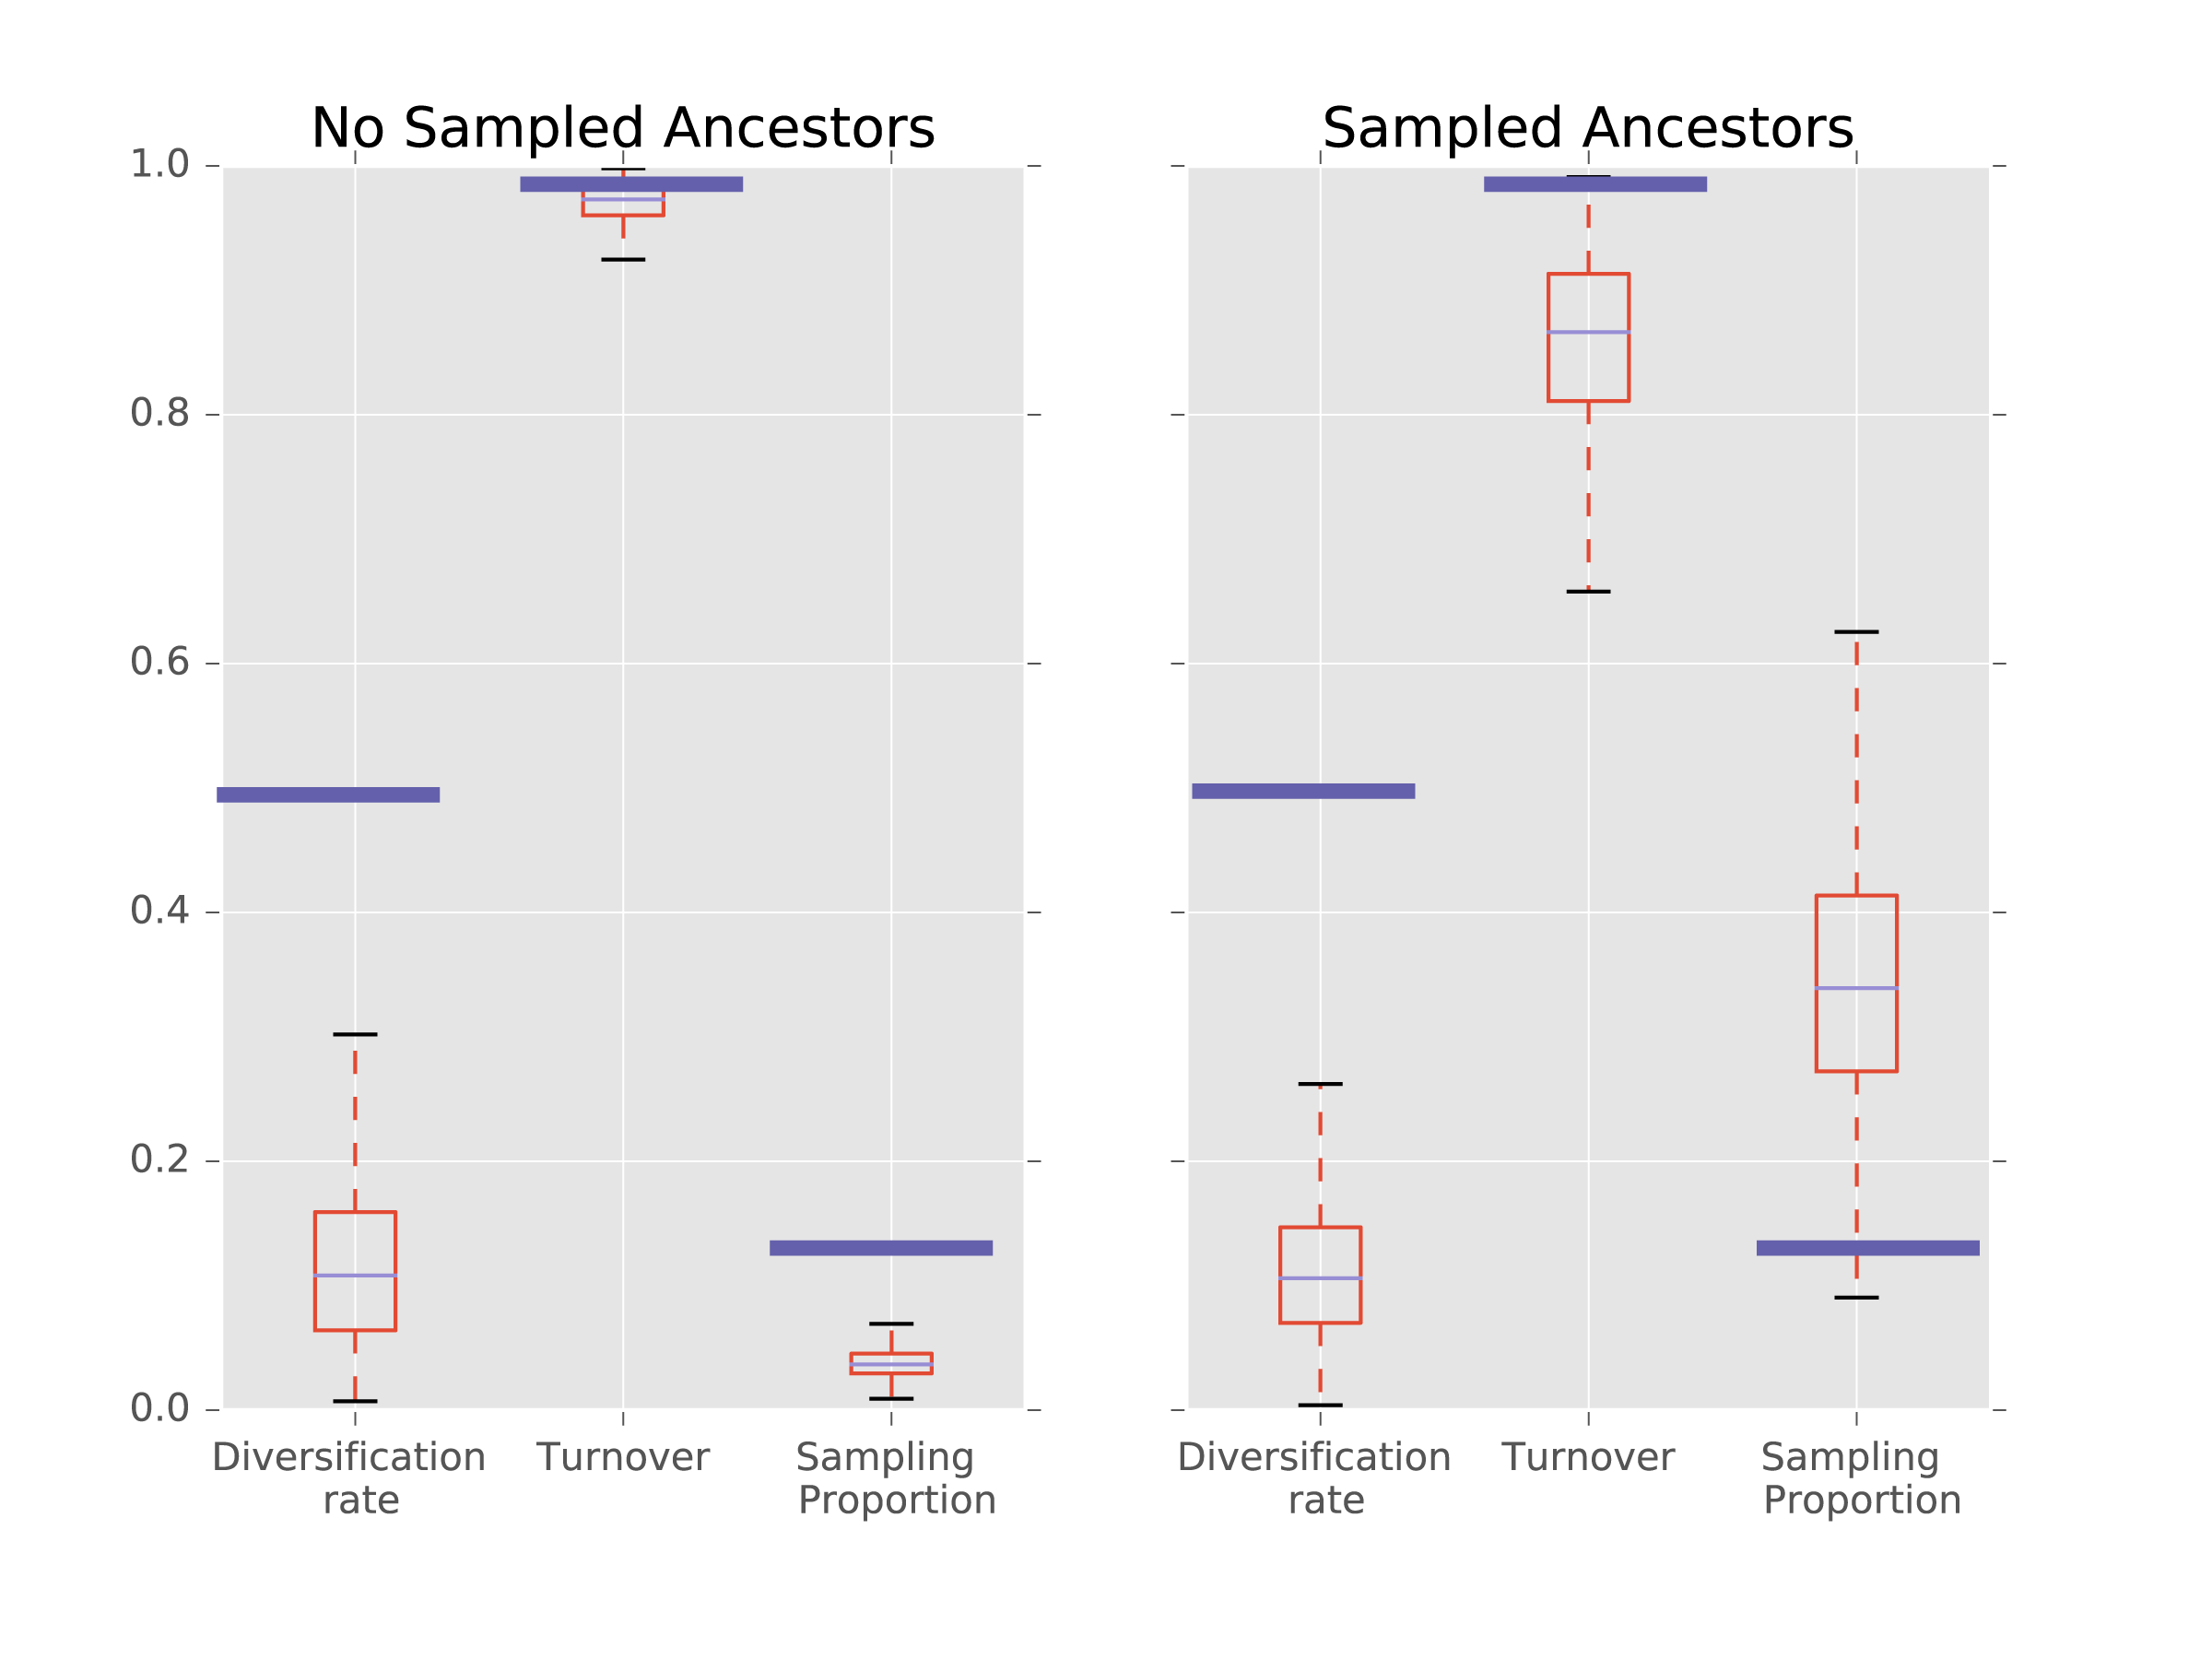
\includegraphics[scale=0.4]{images/HighTurnLowSamplog.png}
\end{figure}
\end{center}
\end{frame}

\begin{frame}
\begin{center}
\begin{figure}
High turnover, low sampling  \\
Few sampled ancestors \\
\lambda   \mu   \psi   \rho \\
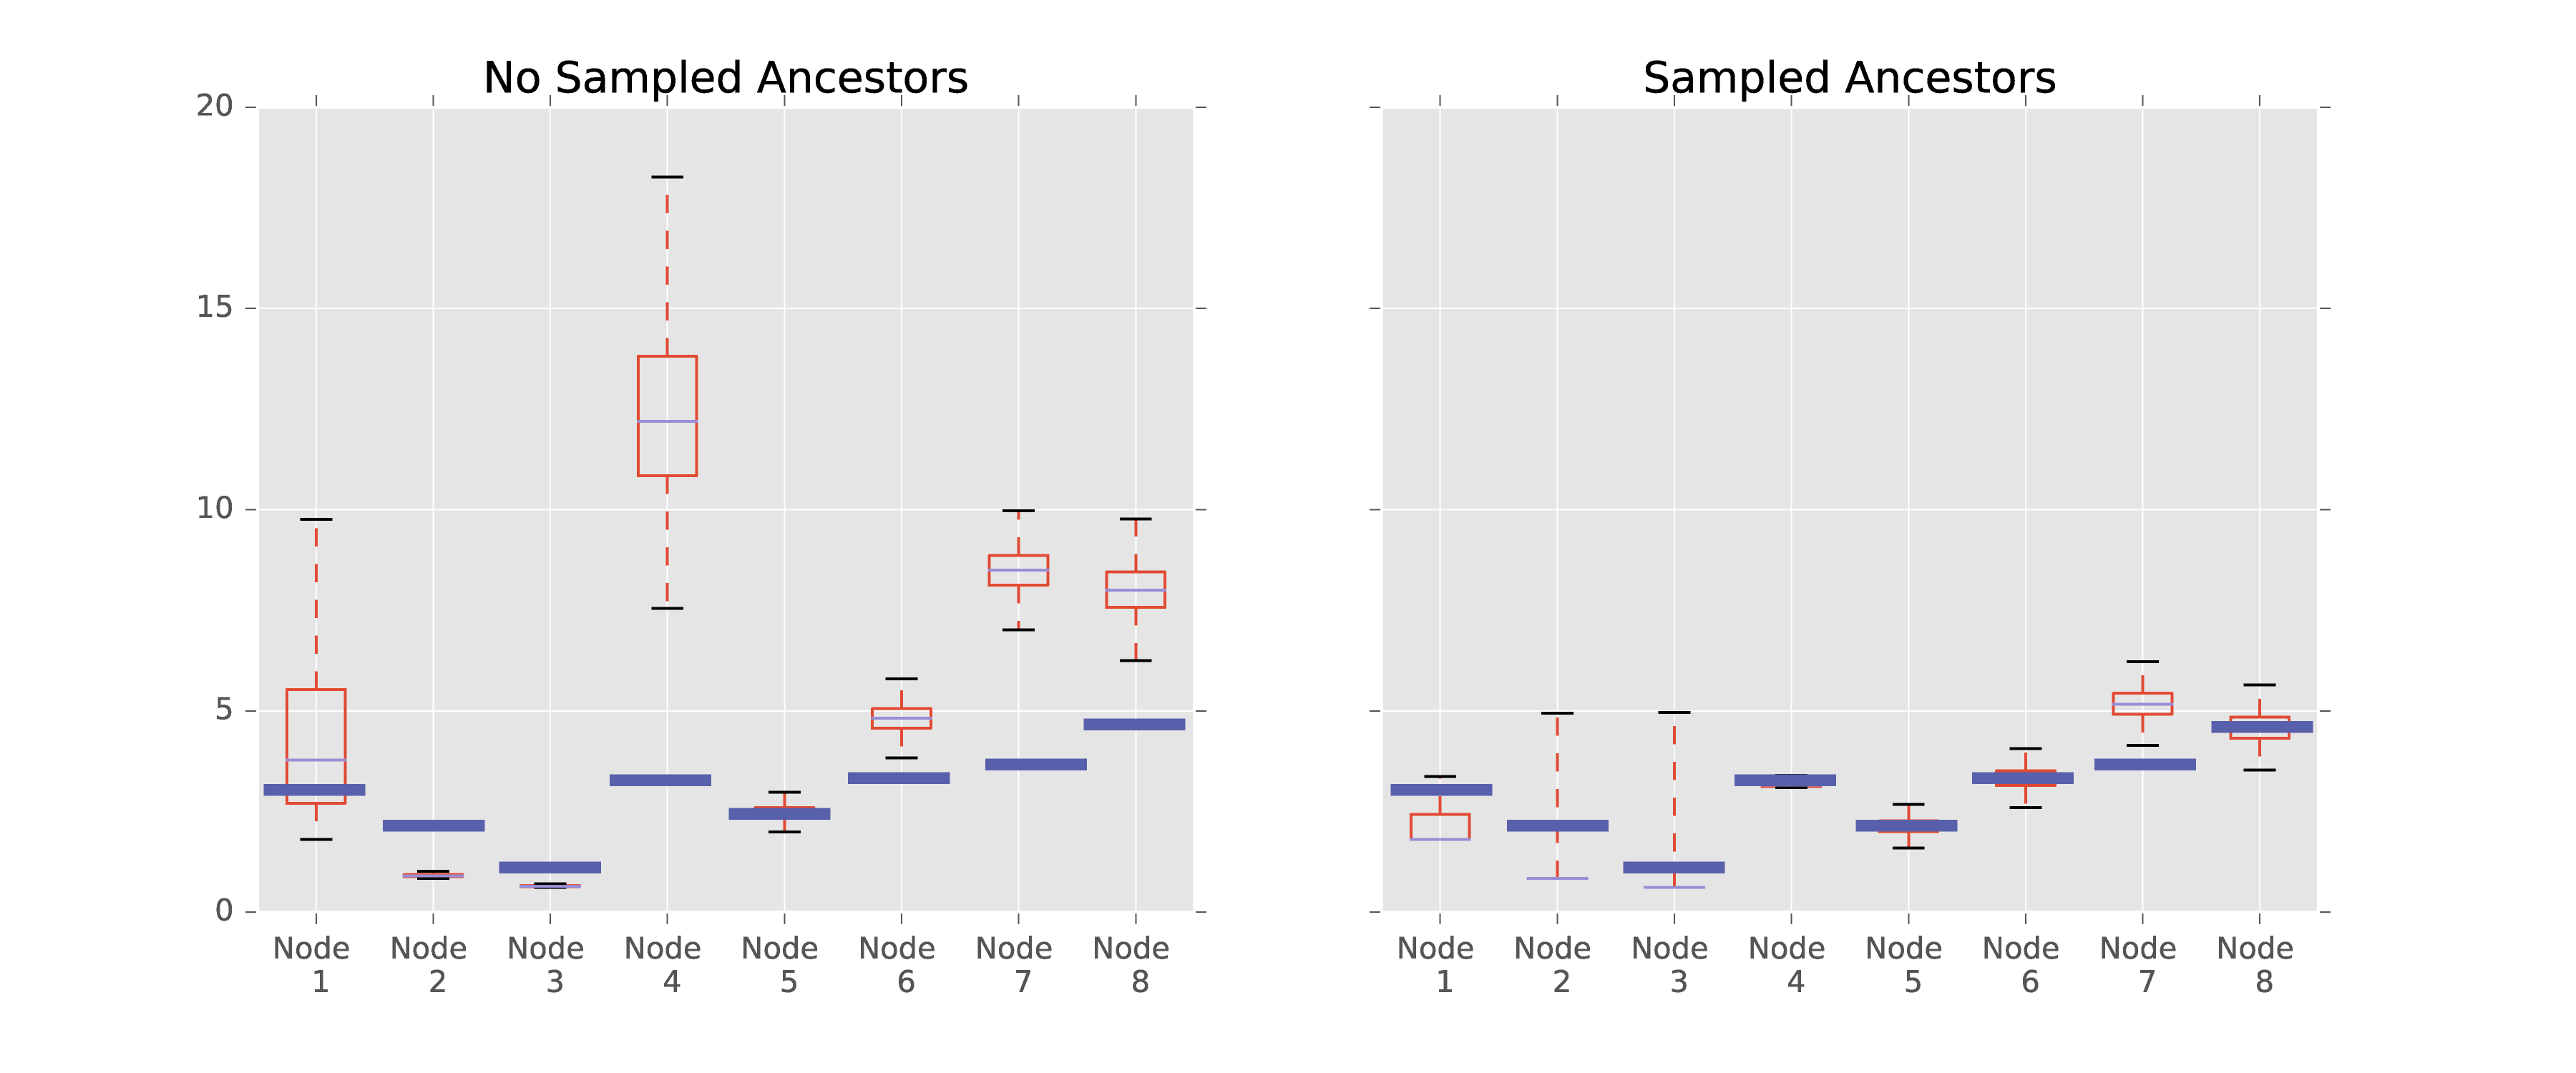
\includegraphics[scale=0.4]{images/HighTurnHighSampnodes.png}
\end{figure}
\end{center}
\end{frame}

\begin{frame}
\frametitle{Results}
\begin{center}
\begin{figure}
Low turnover, high sampling  \\
Few sampled ancestors \\
\lambda   \mu   \psi   \rho \\
\includegraphics[scale=0.4]{images/HighTurnHighSamplog.png}
\end{figure}
\end{center}
\end{frame}


\end{document}